\chapter{Neural Network Training}
\section{Convolutional Neural Networks}	
CNN is trained to predict corresponding a Chinese simplified character given an oracle picture that it represents. It is essential since it acts as a part of a generator or a discriminator in the CycleGAN later. Part oracle pictures of a word are used to train and part pictures of the same characters are used to test the model.

\subsection{Dataset Selection and Processing}
Initially, due to the hardware restriction, in the script \texttt{CNN.py}, only 5043 random chosen oracle pictures whose sizes are 80px$ \times $80px are used to form the neural network, including 4004 (about 80\%) training data and 1039 (about 20\%) testing data of the same 83 Chinese characters. Each one of those characters acts as an individual class labelled as a one-hot vector. The inputs of the neural network are oracle bone script pictures and the outputs of the neural network are probability vectors. A byte with the highest probability labelled which one of 83 characters is the meaning of the oracle picture. And later we used Gaussian filtering and labelling to reduce noise and applied affine transformation and thinning algorithm to extract the skeleton\cite{meng2017recognition}.

\subsection{Network Construction}
There are four steps in total and the structure of CNN is shown in Figure \ref{fig:CNN}.
\begin{figure}[h]
	\centering
	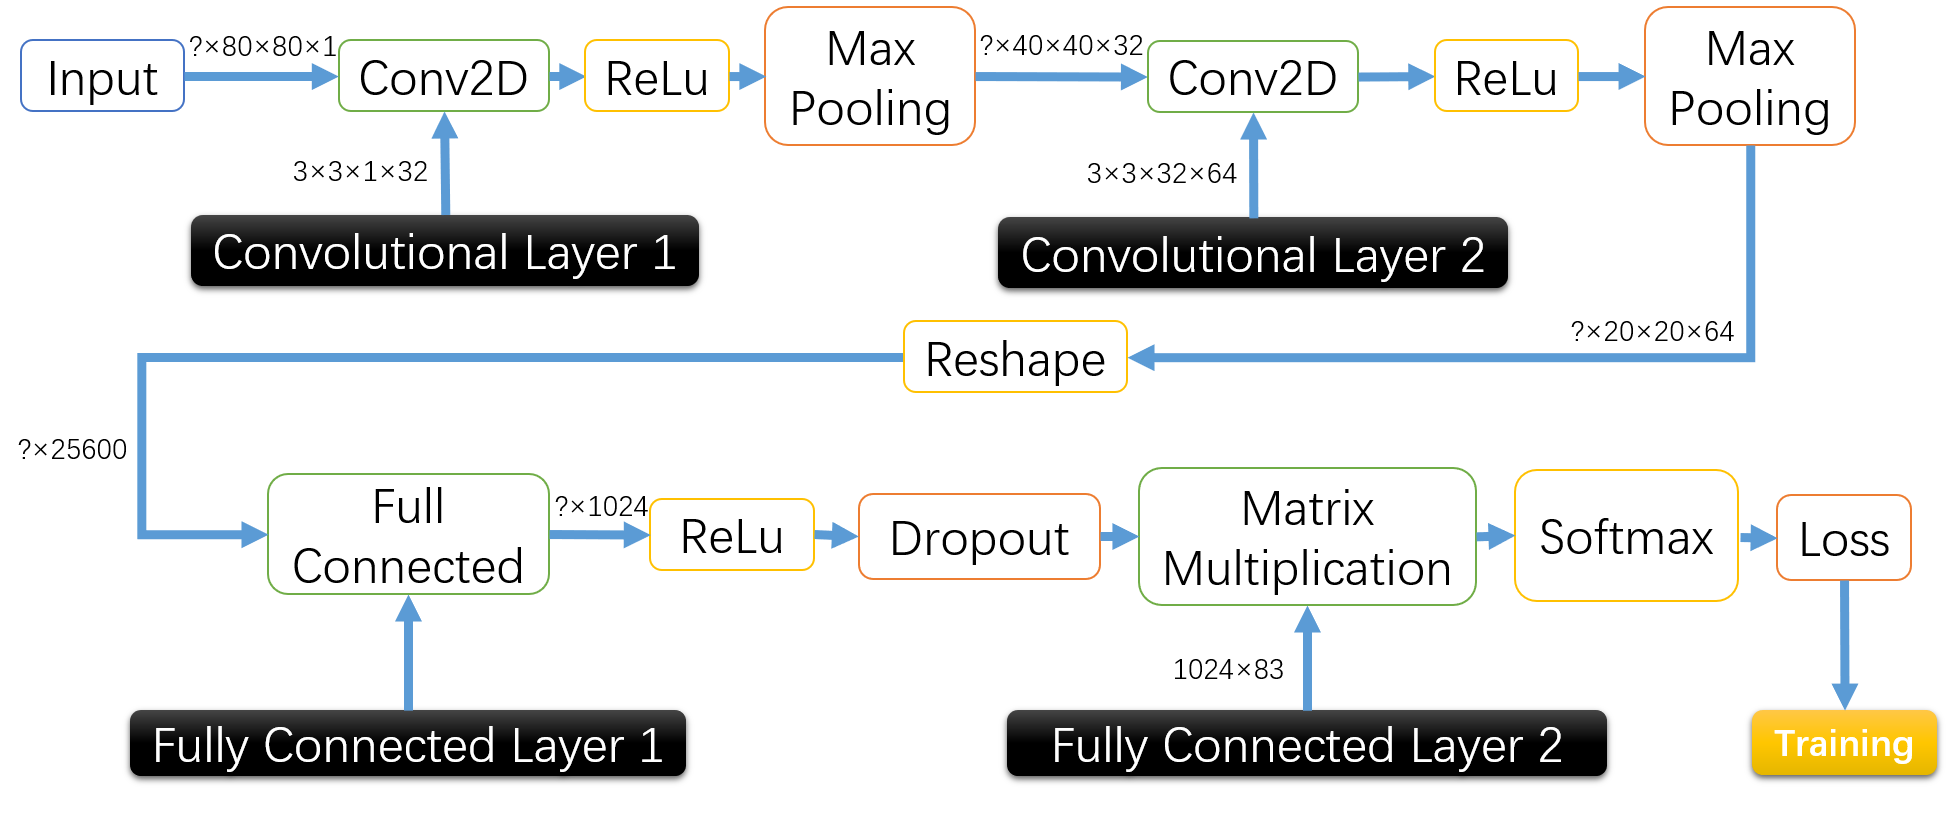
\includegraphics[width=\linewidth]{CNN.png}
	\caption{Structure of convolutional neural networks}
	\label{fig:CNN}
\end{figure}

\begin{itemize}
\item \textbf{Step 1} Load training oracle pictures as a matrix made up of binary numbers, since oracle pictures used here are only monochrome.
\item \textbf{Step 2} Construct a Convolutional Neural Network with two convolutional layers using 3$ \times $3 filters, followed by an activation function ReLU each layer. After that, a 2$ \times $2 max pooling layer whose strike is 2 in a row and 2 in a column at once shrinks the matrices to 50\%$ \times $50\%.
\item \textbf{Step 3} Use a fully connected layer to map the matrices to 1024 nodes. Then, use ReLU as the activation function since Professor Krizhevsky found that\cite{Krizhevsky:2012:ICD:2999134.2999257} ReLU, a nonlinearity activation function is several times faster than hyperbolic tangent $ \tanh $. And then drop out 60\% nodes in case overfitting happens. Without dropout, the model can only predict the word which has been trained. According to \cite{Srivastava:2014:DSW:2627435.2670313}, ``the key idea of dropout is to randomly drop units. Dropout prevents units from co-adapting too much.'' After that, map the 1024 nodes to 83 nodes in the second layer which related the input to one character each and the activation function is softmax.
\item \textbf{Step 4} Test cases are put into the neural network to test the accuracy of the network. The neural network reduces the loss and updates the weights and biases in the network.
\end{itemize}

\subsubsection{Results Visualization, Comparison and Parameter Adjusting}
In the project, we changed one variable at a time and compared its testing accuracy and training speed with the first experiment to find out a better group of parameters. TensorBoard is used to record the performance of each pair of parameters. The parameters which were tested are shown as followed:
\begin{enumerate}
	\item Input size
	\item Convolutional Layer number
	\item Drop out parameter
	\item Learning rate
	\item Filter size
\end{enumerate}
The criteria used to measure the performance of those parameters are two: test accuracy and consumed time.

\subsubsection{Result Analysis and Comparison}
Figure \ref{fig:accuracy} shows the results of seven experiments above and summaries the facts below.
\begin{figure}[h]
	\centering
	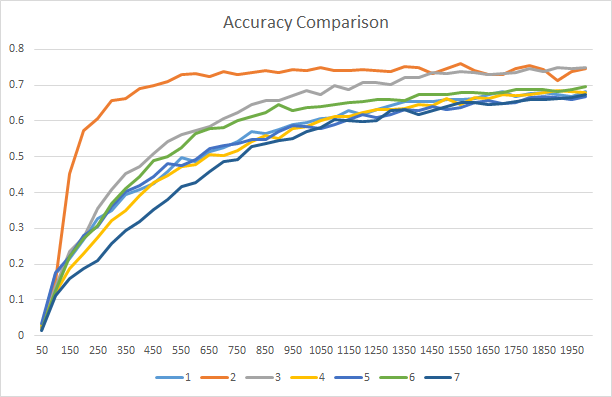
\includegraphics[width=\linewidth]{CNN_Accuracy.png}
	\caption{Test accuracy of 7 experiments}
	\label{fig:accuracy}
\end{figure}
\begin{enumerate}
	\item \textbf{Learning rate in Experiment 1 and 2} When the learning rate was raised from 0.0001 to 0.0005, the consumed time decreased greatly, and the accuracy has been increased. But it is a pity that it is found quite late, so the remaining experiments are conducted using 0.0001 as the learning rate. Using 0.0005 as learning rate can maintain the accuracy at the end, and it also accelerate the training process.
	\item \textbf{Convolutional Layer number in Experiment 1 and 3} Change the convolutional layer from 2 to 3 greatly enhanced the accuracy of the network by 10\% in the end, though the consumed time is increased as well. So it suggests that the deeper neural network (3 layers) has, the better accuracy is achieved when testing.
	\item \textbf{Dropout parameters in Experiment 1, 4 and 5} Dropout is used to prevent the network from overfitting. It drops out some nodes from the first fully connected layer to predict some unknown output using untrained input. Paper \cite{Krizhevsky:2012:ICD:2999134.2999257} mentioned that when using 0.5 as dropout rate, learning can have better performance: ``The neurons which are ``dropped out'' in this way do not contribute to the forward pass and do not participate in backpropagation.'' But in this neural network, the difference of performance does not very obvious with dropout rate varying from 0.5 to 0.6.
	\item \textbf{Filter size in Experiment 1 and 6} The filter size means the view of a computer when scanning the numbers of features in a neural network. A bigger filter size indicates that the machine can ``see'' and catches a bigger feature.
	\item \text{Input size in Experiment 1 and 7} Original Oracle pictures from the website are adjusted without shape transformation. Two versions of the picture adjusting scripts change the size from 80px$ \times $80px to 100px$ \times $100px. The time consumed when a single picture is 100px$ \times $100px increased by 18.83\%, while the accuracy even decreased a little bit. It suggests that there is no need to increase the size of pictures from 80px$ \times $80px pixels to 100px$ \times $100px.
\end{enumerate}

\section{Conditional Generative Adversarial Networks}
Before we actually apply conditional GAN, we have to create a unique dataset for it. After doing statistics for both bronze and oracle bone script dataset, we found that 666 individual characters (recorded in \texttt{Unique\_Characters.txt} file) co-appear in both datasets and each one contains at least one and up to hundreds of different images. For each character, we chose one image to represent it in our paired dataset randomly and two folder with exactly 666 files were created. And then we run the script \texttt{Tools/process.py} to generate image pairs for CGAN training.
\begin{lstlisting}[language = bash, caption = Image Pair Generation]
python3 Tools/process.py \
--input_dir ORACLE \
--b_dir BRONZE \
--operation combine \
--output_dir OUTPUT
\end{lstlisting}
\begin{figure}[h]
	\centering
	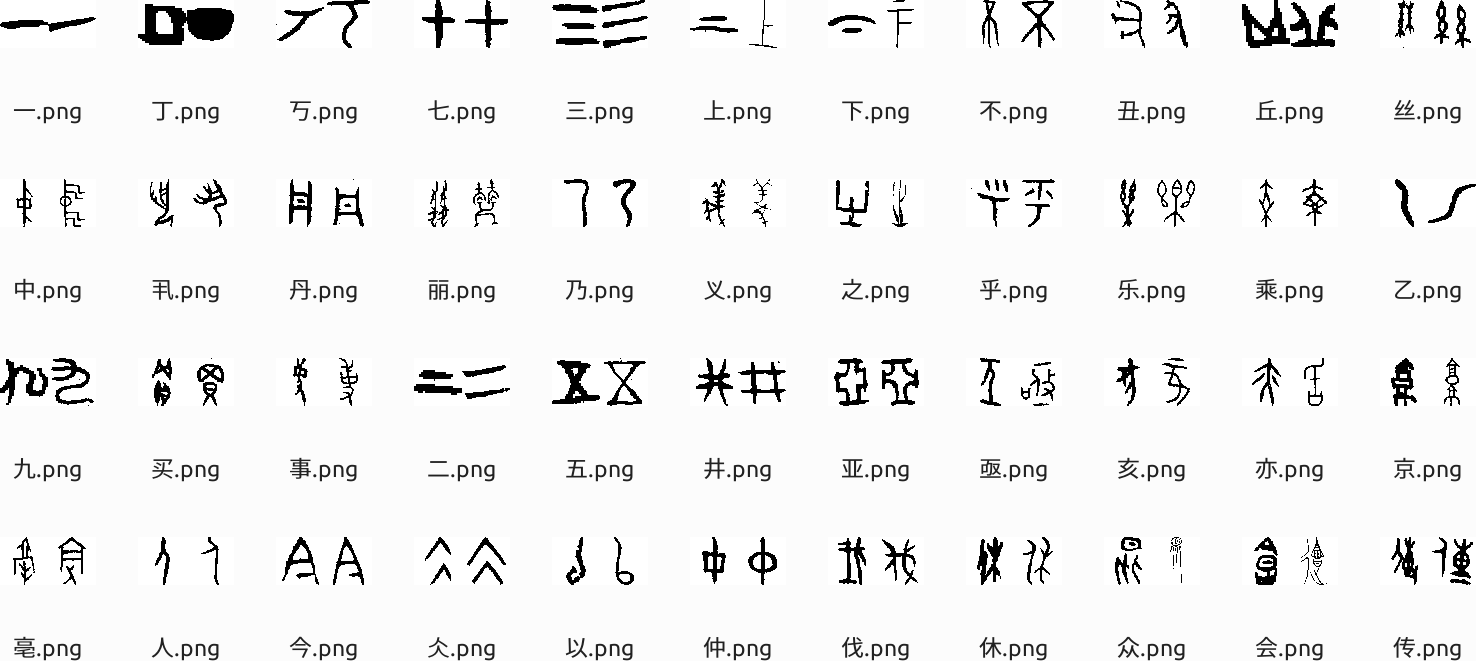
\includegraphics[width=\linewidth]{CGAN_Training_W.png}
	\caption{Samples from Initial Failure}
	\label{fig:failure}
\end{figure}
And then we divided them into training set and validation test with threshold 80\% respectively, which means that there are 532 samples in training set and correspondingly there are 134 ones in validation set (partly showed in Figure \ref{fig:failure}). After several experiments with relatively small epochs (less than 20), we found unfortunately that it did not work because all generated images were purely white, which indicates that in order to create real enough photos, generators learn from input images whose most part is white background. So we had to do some refinements for images to avoid this issues. And the most intuitive approach coming to our mind after a brief brainstorm is to change background of each image.
\begin{figure}[h]
	\centering
	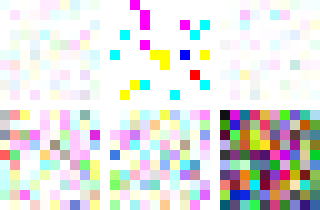
\includegraphics{Noise.png}
	\caption{Samples from 6 different noise distributions (10px$ \times $10px) (first row from left to right: Gaussian, Impulse and Laplacian; second row from left to right: Multiplicative, Poisson and Random)}
	\label{fig:noise}
\end{figure}
And after checking all possible random images from Figure \ref{fig:noise}, we realised that the simplest ``Random'' distribution may be the most useful in our case. And to avoid letting noise pixels appear on actual monochrome characters, we made the background of character image transparent and merged it to a new noise-processed background (which is showed in Figure \ref{fig:CGAN_training}).
\begin{figure}[h]
	\centering
	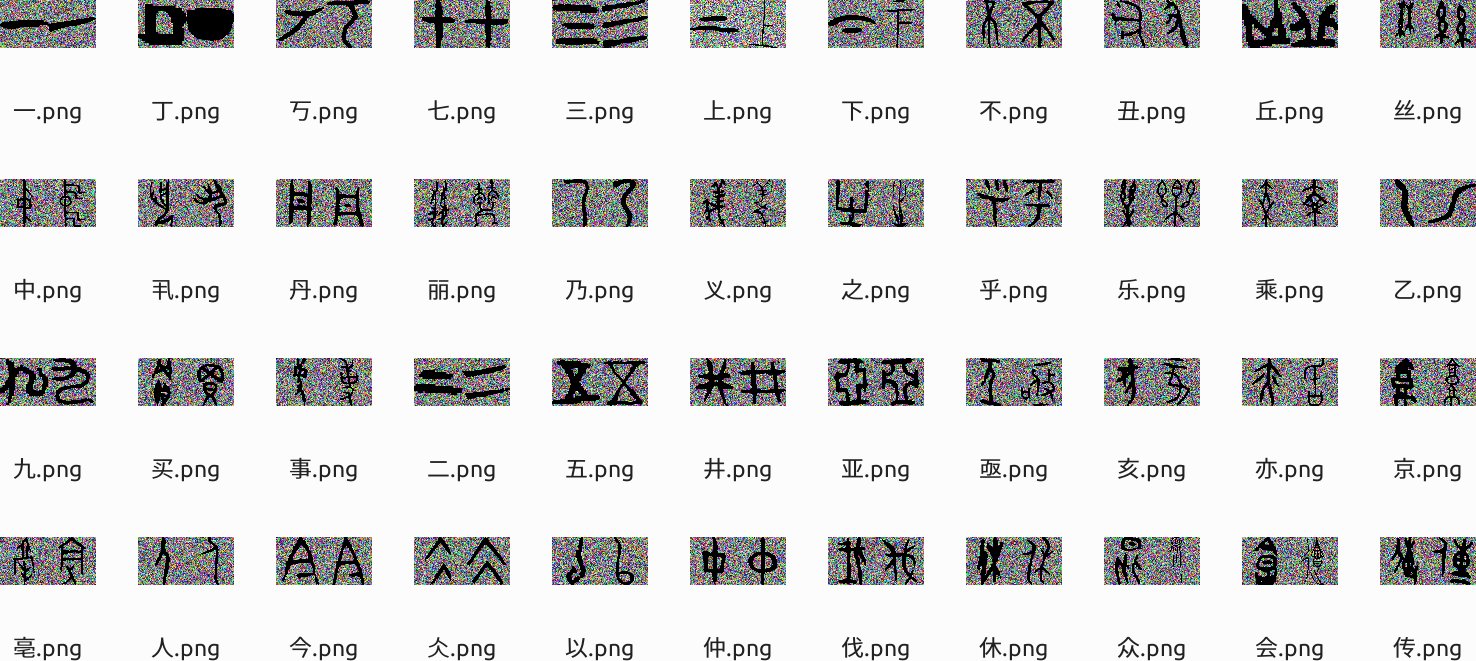
\includegraphics[width=\linewidth]{CGAN_Training_R.png}
	\caption{Samples from CGAN training dataset}
	\label{fig:CGAN_training}
\end{figure}

We started our training with batch size = 32, learning rate = 0.0002 and maximum epoch = 200. Part of results can be seen in Appendix \ref{ch:appendix_2} and more validation results are available on our GitHub repository. Obviously, current results are not ideal, so we continued to train our CGAN models with much more epochs (5000 and 20000, which are listed in Appendix \ref{ch:appendix_3} and \ref{ch:appendix_4} separately.

Eventually, according to GAN Zoo\footnote{\url{https://github.com/hindupuravinash/the-gan-zoo}}, there are hundreds of different GANs available. We also went through some of them and found potential ones to be our next candidates.